\documentclass{standalone}
\usepackage{tikz}
\usetikzlibrary{patterns, positioning}


\begin{document}
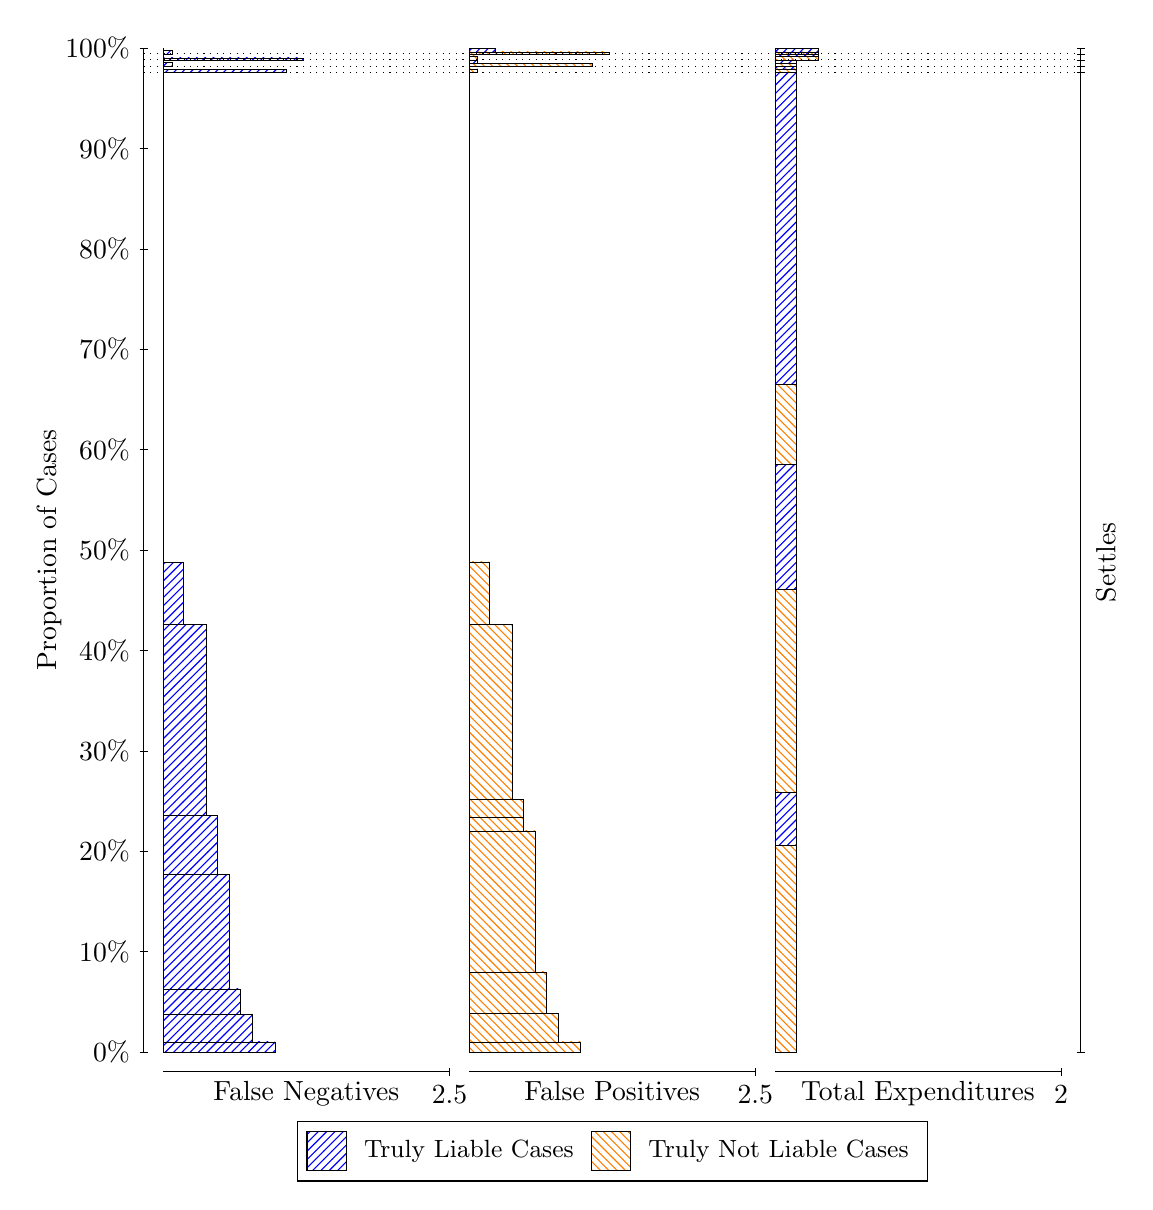
\begin{tikzpicture}
\draw[black, very thin] (1.5,1.75) -- (1.5,14.5);
\node[rotate=90, text=black, anchor=center] at (0.3, 8.125) {Proportion of Cases};
\draw[black, very thin] (1.45,1.75) -- (1.55,1.75);
\node[text=black, anchor=east] at (1.45, 1.75) {0\%};
\draw[black, very thin] (1.45,3.025) -- (1.55,3.025);
\node[text=black, anchor=east] at (1.45, 3.025) {10\%};
\draw[black, very thin] (1.45,4.3) -- (1.55,4.3);
\node[text=black, anchor=east] at (1.45, 4.3) {20\%};
\draw[black, very thin] (1.45,5.575) -- (1.55,5.575);
\node[text=black, anchor=east] at (1.45, 5.575) {30\%};
\draw[black, very thin] (1.45,6.85) -- (1.55,6.85);
\node[text=black, anchor=east] at (1.45, 6.85) {40\%};
\draw[black, very thin] (1.45,8.125) -- (1.55,8.125);
\node[text=black, anchor=east] at (1.45, 8.125) {50\%};
\draw[black, very thin] (1.45,9.4) -- (1.55,9.4);
\node[text=black, anchor=east] at (1.45, 9.4) {60\%};
\draw[black, very thin] (1.45,10.675) -- (1.55,10.675);
\node[text=black, anchor=east] at (1.45, 10.675) {70\%};
\draw[black, very thin] (1.45,11.95) -- (1.55,11.95);
\node[text=black, anchor=east] at (1.45, 11.95) {80\%};
\draw[black, very thin] (1.45,13.225) -- (1.55,13.225);
\node[text=black, anchor=east] at (1.45, 13.225) {90\%};
\draw[black, very thin] (1.45,14.5) -- (1.55,14.5);
\node[text=black, anchor=east] at (1.45, 14.5) {100\%};

\draw[black, very thin] (13.4,1.75) -- (13.4,14.5);
\draw[black, very thin] (13.35,1.75) -- (13.45,1.75);
\node[anchor=west] at (13.35, 1.75) {};
\draw[black, very thin] (13.35,14.192) -- (13.45,14.192);
\node[anchor=west] at (13.35, 14.192) {};
\draw[black, very thin] (13.35,14.27) -- (13.45,14.27);
\node[anchor=west] at (13.35, 14.27) {};
\draw[black, very thin] (13.35,14.35) -- (13.45,14.35);
\node[anchor=west] at (13.35, 14.35) {};
\draw[black, very thin] (13.35,14.425) -- (13.45,14.425);
\node[anchor=west] at (13.35, 14.425) {};
\draw[black, very thin] (13.35,14.5) -- (13.45,14.5);
\node[anchor=west] at (13.35, 14.5) {};

\draw[black, very thin, pattern color=blue, pattern=north east lines] (1.75,1.75) rectangle (3.167,1.8773);
\draw[black, very thin, pattern color=blue, pattern=north east lines] (1.75,1.8773) rectangle (2.8763,2.2235);
\draw[black, very thin, pattern color=blue, pattern=north east lines] (1.75,2.2235) rectangle (2.731,2.5514);
\draw[black, very thin, pattern color=blue, pattern=north east lines] (1.75,2.5514) rectangle (2.5857,4.0056);
\draw[black, very thin, pattern color=blue, pattern=north east lines] (1.75,4.0056) rectangle (2.4403,4.7532);
\draw[black, very thin, pattern color=blue, pattern=north east lines] (1.75,4.7532) rectangle (2.295,7.1759);
\draw[black, very thin, pattern color=blue, pattern=north east lines] (1.75,7.1759) rectangle (2.0043,7.9689);
\draw[black, very thin, pattern color=orange, pattern=north west lines] (1.75,7.9689) rectangle (1.75,14.192);
\draw[black, very thin, pattern color=blue, pattern=north east lines] (1.75,14.192) rectangle (3.3123,14.226);
\draw[black, very thin, pattern color=orange, pattern=north west lines] (1.75,14.226) rectangle (1.75,14.27);
\draw[black, very thin, pattern color=blue, pattern=north east lines] (1.75,14.27) rectangle (1.859,14.316);
\draw[black, very thin, pattern color=orange, pattern=north west lines] (1.75,14.316) rectangle (1.75,14.35);
\draw[black, very thin, pattern color=blue, pattern=north east lines] (1.75,14.35) rectangle (3.5303,14.376);
\draw[black, very thin, pattern color=orange, pattern=north west lines] (1.75,14.376) rectangle (1.75,14.425);
\draw[black, very thin, pattern color=blue, pattern=north east lines] (1.75,14.425) rectangle (1.859,14.474);
\draw[black, very thin, pattern color=orange, pattern=north west lines] (1.75,14.474) rectangle (1.75,14.5);
\draw[black, very thin, pattern color=orange, pattern=north west lines] (5.6333,1.75) rectangle (7.0503,1.8769);
\draw[black, very thin, pattern color=orange, pattern=north west lines] (5.6333,1.8769) rectangle (6.7597,2.2443);
\draw[black, very thin, pattern color=orange, pattern=north west lines] (5.6333,2.2443) rectangle (6.6143,2.768);
\draw[black, very thin, pattern color=orange, pattern=north west lines] (5.6333,2.768) rectangle (6.469,4.5588);
\draw[black, very thin, pattern color=orange, pattern=north west lines] (5.6333,4.5588) rectangle (6.3237,4.7314);
\draw[black, very thin, pattern color=orange, pattern=north west lines] (5.6333,4.7314) rectangle (6.3237,4.9615);
\draw[black, very thin, pattern color=orange, pattern=north west lines] (5.6333,4.9615) rectangle (6.1783,7.1789);
\draw[black, very thin, pattern color=orange, pattern=north west lines] (5.6333,7.1789) rectangle (5.8877,7.9727);
\draw[black, very thin, pattern color=blue, pattern=north east lines] (5.6333,7.9727) rectangle (5.6333,14.192);
\draw[black, very thin, pattern color=orange, pattern=north west lines] (5.6333,14.192) rectangle (5.7423,14.236);
\draw[black, very thin, pattern color=blue, pattern=north east lines] (5.6333,14.236) rectangle (5.6333,14.27);
\draw[black, very thin, pattern color=orange, pattern=north west lines] (5.6333,14.27) rectangle (7.1957,14.304);
\draw[black, very thin, pattern color=blue, pattern=north east lines] (5.6333,14.304) rectangle (5.7423,14.35);
\draw[black, very thin, pattern color=orange, pattern=north west lines] (5.6333,14.35) rectangle (5.7423,14.399);
\draw[black, very thin, pattern color=blue, pattern=north east lines] (5.6333,14.399) rectangle (5.6333,14.425);
\draw[black, very thin, pattern color=orange, pattern=north west lines] (5.6333,14.425) rectangle (7.4137,14.451);
\draw[black, very thin, pattern color=blue, pattern=north east lines] (5.6333,14.451) rectangle (5.9603,14.5);
\draw[black, very thin, pattern color=orange, pattern=north west lines] (9.5167,1.75) rectangle (9.7892,4.3701);
\draw[black, very thin, pattern color=blue, pattern=north east lines] (9.5167,4.3701) rectangle (9.7892,5.0442);
\draw[black, very thin, pattern color=orange, pattern=north west lines] (9.5167,5.0442) rectangle (9.7892,7.6288);
\draw[black, very thin, pattern color=blue, pattern=north east lines] (9.5167,7.6288) rectangle (9.7892,9.2103);
\draw[black, very thin, pattern color=orange, pattern=north west lines] (9.5167,9.2103) rectangle (9.7892,10.228);
\draw[black, very thin, pattern color=blue, pattern=north east lines] (9.5167,10.228) rectangle (9.7892,14.192);
\draw[black, very thin, pattern color=orange, pattern=north west lines] (9.5167,14.192) rectangle (9.7892,14.236);
\draw[black, very thin, pattern color=blue, pattern=north east lines] (9.5167,14.236) rectangle (9.7892,14.27);
\draw[black, very thin, pattern color=orange, pattern=north west lines] (9.5167,14.27) rectangle (9.7892,14.304);
\draw[black, very thin, pattern color=blue, pattern=north east lines] (9.5167,14.304) rectangle (9.7892,14.35);
\draw[black, very thin, pattern color=orange, pattern=north west lines] (9.5167,14.35) rectangle (10.062,14.399);
\draw[black, very thin, pattern color=blue, pattern=north east lines] (9.5167,14.399) rectangle (10.062,14.425);
\draw[black, very thin, pattern color=orange, pattern=north west lines] (9.5167,14.425) rectangle (10.062,14.451);
\draw[black, very thin, pattern color=blue, pattern=north east lines] (9.5167,14.451) rectangle (10.062,14.5);
\draw[black, dotted] (1.5,14.192) -- (13.4,14.192);
\draw[black, dotted] (1.5,14.27) -- (13.4,14.27);
\draw[black, dotted] (1.5,14.35) -- (13.4,14.35);
\draw[black, dotted] (1.5,14.425) -- (13.4,14.425);
\draw[black, very thin] (1.75,1.5) -- (5.3833,1.5);
\node[text=black, anchor=north] at (3.5667, 1.5) {False Negatives};
\draw[black, very thin] (5.3833,1.45) -- (5.3833,1.55);
\node[text=black, anchor=north] at (5.3833, 1.45) {2.5};

\draw[black, very thin] (5.6333,1.5) -- (9.2667,1.5);
\node[text=black, anchor=north] at (7.45, 1.5) {False Positives};
\draw[black, very thin] (9.2667,1.45) -- (9.2667,1.55);
\node[text=black, anchor=north] at (9.2667, 1.45) {2.5};

\draw[black, very thin] (9.5167,1.5) -- (13.15,1.5);
\node[text=black, anchor=north] at (11.333, 1.5) {Total Expenditures};
\draw[black, very thin] (13.15,1.45) -- (13.15,1.55);
\node[text=black, anchor=north] at (13.15, 1.45) {2};

\node[text=black, centered, rotate=90] at (13.72, 7.9708) {Settles};





\draw (7.449999999999999,1.5) node[draw=none] (baseCoordinate) {};
\begin{scope}[align=center]
        \matrix[scale=0.5, draw=black, below=0.5cm of baseCoordinate, nodes={draw}, column sep=0.1cm]{
            \node[rectangle, draw, minimum width=0.5cm, minimum height=0.5cm, pattern color=blue, pattern=north east lines] {}; &
            \node[draw=none, font=\small, text=black] (B) {Truly Liable Cases}; &
            \node[rectangle, draw, minimum width=0.5cm, minimum height=0.5cm, pattern color=orange, pattern=north west lines] {}; &
            \node[draw=none, font=\small, text=black] (B) {Truly Not Liable Cases}; \\
            };
\end{scope}

\end{tikzpicture}
\end{document}